% This file was created by tikzplotlib v0.9.2.
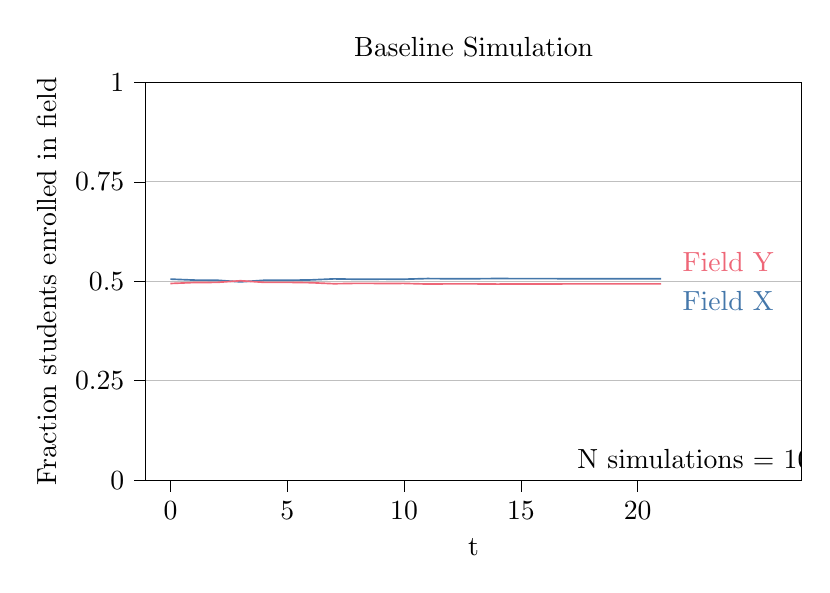
\begin{tikzpicture}

\definecolor{color0}{rgb}{0.266666666666667,0.466666666666667,0.666666666666667}
\definecolor{color1}{rgb}{0.933333333333333,0.4,0.466666666666667}

\begin{axis}[
height=6.6314113761540705cm,
tick align=outside,
tick pos=left,
title={Baseline Simulation},
width=9.904475999999999cm,
x grid style={white!69.0196078431373!black},
xlabel={t},
xmin=-1.05, xmax=27,
xtick style={color=black},
xtick={0,5,10,15,20},
xticklabels={\(\displaystyle 0\),\(\displaystyle 5\),\(\displaystyle 10\),\(\displaystyle 15\),\(\displaystyle 20\)},
ylabel={Fraction students enrolled in field},
ymajorgrids,
ymin=0, ymax=1,
ytick style={color=black},
ytick={0,0.25,0.5,0.75,1},
yticklabels={\(\displaystyle 0\),\(\displaystyle 0.25\),\(\displaystyle 0.5\),\(\displaystyle 0.75\),\(\displaystyle 1\)}
]
\addplot [semithick, color0]
table {%
0 0.505500078201294
1 0.503099918365479
2 0.502699971199036
3 0.498600006103516
4 0.502599954605103
5 0.502599954605103
6 0.503499984741211
7 0.506099939346313
8 0.505100011825562
9 0.505399942398071
10 0.505300045013428
11 0.506900072097778
12 0.506399989128113
13 0.506500005722046
14 0.506999969482422
15 0.506700038909912
16 0.506799936294556
17 0.506500005722046
20 0.506500005722046
21 0.506500005722046
};
\addplot [semithick, color1]
table {%
0 0.494500041007996
1 0.496899962425232
2 0.497300028800964
3 0.501399993896484
4 0.497400045394897
5 0.497400045394897
6 0.496500015258789
7 0.493900060653687
8 0.494899988174438
9 0.494600057601929
10 0.494699954986572
11 0.493099927902222
12 0.493600010871887
13 0.493499994277954
14 0.493000030517578
15 0.493299961090088
16 0.493200063705444
17 0.493499994277954
20 0.493499994277954
21 0.493499994277954
};
\draw (axis cs:21.5,0.4265) node[
  anchor=base west,
  text=color0,
  rotate=0.0
]{Field X};
\draw (axis cs:21.5,0.5235) node[
  anchor=base west,
  text=color1,
  rotate=0.0
]{Field Y};
\draw (axis cs:17,0.03) node[
  anchor=base west,
  text=black,
  rotate=0.0
]{N simulations = 10,000};
\end{axis}

\end{tikzpicture}
